\documentclass[11pt]{article}

\usepackage[margin=25mm,a4paper]{geometry}

\setlength{\parindent}{0em}
\setlength{\parskip}{1em}

\title{The use of Distributed Tracing in the Maintenance phase\\of the Software Development Life Cycle}

\author{Nicola M\"{o}ssner \\ 2268685m}

\date{17. January 2020}

\usepackage[numbers]{natbib}
\usepackage{graphicx}
\usepackage{float}

\begin{document}

\maketitle

\section{Background}

% A background, including a general description of the context of the problem and relevance to the industry partner.

When reflecting on the Software Development Life Cycle (SDLC) of different projects I have personally been involved in, observed, or read about, it becomes apparent to me that the last stage which is often described as the 'Maintenance phase' forms a major part of the whole software development process.

Maintenance involves various disciplines, such as: % TODO: Maybe reference https://www.econnectivity.se/app-maintenance-cost-can-be-three-times-higher-than-development-cost/
\begin{itemize}
    \item Correcting issues/bugs in the code.
    \item Adapting the behaviour of the application to meet changing and evolving requirements.
    \item Enhancing the performance of the software to improve user experience and satisfaction.
    \item Updating technologies, platforms, frameworks, and infrastructure to keep up with the latest standards and innovations, and making necessary changes to the software accordingly.
    \item Monitoring and analysing the behaviour and performance of the software.
\end{itemize}
It is in fact widely known and agreed on that the maintenance cost far exceeds the development costs for most software projects. In the article \textit{Frequently Forgotten Fundamental Facts about Software Engineering} \cite{ieeesoftware} published in the \textit{IEEE Software} scientific journal, Robert L. Glass proposes that on average maintenance consumes about 60\% of software costs. Other sources affirm this theory and come to a consensus illustrated roughly in the following diagram:

\begin{figure}[H]
    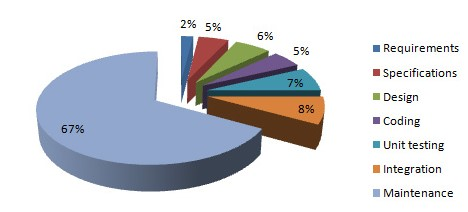
\includegraphics[width=11cm]{maintenance_costs}
    \centering
    \caption{Approximate Software Life Cycle Costs}
    \label{fig:maintenance_costs}
\end{figure}

Maintaining and improving an existing software application/solution consumes a vast amount of resources and this is no different at my current employer, ResDiary.

ResDiary provides its customers with a reservation and table management system for the hospitality sector. The nature of this industry demands highly available and well performing software solutions. Lacking in those areas can result in a loss of profit for our customers. For this reason, we are constantly monitoring and enhancing the stability and performance of the services we provide.

To improve the process of pinpointing potential areas of improvement, we are eager to introduce \textit{Distributed Tracing} to our applications.
\begin{quote}
    "Distributed tracing helps pinpoint where failures occur and what causes poor performance." \cite{opentracing}
\end{quote}  
With this in mind, we expect this method to assist us in identifying issues in our software that we can address either with an immediate quick fix or with a complete overhaul of a particular software component, SQL query, etc.

\section{Problem Description}

% An explanation of the nature of the problem to be addressed, the symptoms, the extent of the problem (is it specific to
% your employer, a sector, or the wider software industry?), and associated evidence in support of your description of the
% problem (conversations with team members, literature, personal diary entries).

\subsection{The nature of the problem}

With the growing trend of microservices, orchestrated into large-scale applications, it becomes more challenging to trace errors in the code, to spot bottlenecks and slow parts of the application, to find buggy code or simply to find areas of improvement. For example, when a request to a web application takes longer than expected, it is difficult to determine if this was caused by part of the application code, a database query, some code in another application that the request gets routed to or a call to a third-party library.

At ResDiary we currently have no distinct approach to investigate the cause for slow or failing requests. At the moment we resort to log messages and graphs depicting the health and/or uptime of components and infrastructure. This approach can be very broad and slow as it takes time to pin down the exact nature of an issue and may involve some guesses and investigation into a wrong direction at first. 

\subsection{The symptoms}

Doing this kind of investigation into incidents often requires multiple people to get involved. A recent incident I can recall got three members of my team involved, the team leader to check the logs produced by our application, the database administrator to check the SQL query store for any signs of poor performing queries, and another to go through the logs of our infrastructure, namely the Kubernetes resources which are hosting the application.\\
This is not ideal, consuming precious time that could have been spent elsewhere.

When it comes to a support incident that affects customers directly it is crucial to resolve the situation promptly or at least release a status update as to the nature of the problem and the approximate expected duration of the incident. Currently, the response time fluctuates widely due to the aforementioned reason of potentially long investigation times.

From my weekly diary entries, I take another example of a symptom. As part of some improvement work, we did some SQL query tuning to increase the performance of a query. At the same time, we altered the code slightly so that the query itself was executed fewer times. Both changes went out in the same release. It was then difficult to say if the changes had the expected positive impact on the users' requests as there are many components involved in a request. We monitored the performance over some time and could conclude that overall, the request time did reduce as anticipated. But even then, it was almost impossible to say which of the two changes had made a bigger impact.

Having the ability to trace an incoming request from start to finish, and measuring how much time it takes within the different components and perhaps even functions and methods of the whole application would expose root causes for failing or slow requests much quicker.\\
It would expectedly require less working hours and people to fix issues. On-call developers would be able to resolve incidents faster and minimise customer impact. Changes made to existing software could be monitored and evaluated with reduced effort and time.

\subsection{Evidence in support of the problem}

% TODO: Evidence in support of problem description.

\subsection{Extent of the problem}

A majority of software projects involve a Maintenance phase of some form or another and will therefore face this problem sooner or later. The specifics of the symptoms may differ across software solutions, but in general, there will be similarities in the process of dealing with them.\\
In some cases, no further actions are required as improving the software is not necessary for different reasons so no monitoring or investigations are undertaken but for most projects, I think further improvements are essential to stay competitive and provide a secure product.

\section{Objectives} 

% Give the set of objectives describing the outcomes of the project, either in terms of knowledge acquired through
% experimentation or artefacts delivered (including software code, data sets, process documentation, for example).  These
% objectives will specify the *Definition of Done* for the overall project.

The choice of an appropriate Tracing Framework is part of the Work Plan (see section \ref{WorkPlan}), hence for now, I will refer to it as \textit{Tracing Framework}. Possible choices are \textit{OpenTracing} and \textit{.NET Core 3.0 Diagnostics}.

In the same manner, I will refer to the eventual implementation choice of the Distributed Tracing System such as \textit{Jaeger} or \textit{ZipKin} simply as \textit{Distributed Tracing System}.

The following objectives are to be completed within the scope of this project:

\textbf{1.} The Tracing Framework is implemented in our \textit{.NET Core} applications.

    % How do we do this?
    % Add some code to our existing apps or have an extra app for this?
    % Only to the ones running in Kubernetes?
    % Use OpenTracing or .NET Core 3.0 Diagnostics?

\textbf{2.} Delivered a \textit{helm chart}\cite{helmcharts} for the Distributed Tracing System that can be deployed locally and to Azure Kubernetes Services (AKS).

\textbf{3.} The Distributed Tracing System is running in the ResDiary AKS staging cluster.

\textbf{4.} The Distributed Tracing System is running in the ResDiary AKS production cluster.

\textbf{5.} Traces gathered through the Tracing Framework are visualised meaningfully in the Distributed Tracing System.

\textbf{6.} Delivered an experience report from the DevOps team and on-call developers at ResDiary, discussing some of the following concerns:
\begin{itemize}
    \item How has this new approach affected the process of finding issues in general?
    \item How has it affected the time to get to the bottom of (and resolve) an on-call support incident?
    \item Does this additional tool increase your confidence to track and resolve issues while on-call or in your everyday work?
    \item Does the data gathered and depicted in the Distributed Tracing System provide useful indications for areas of improvement?
\end{itemize}

\section{Work Plan}
\label{WorkPlan}

% Describe the overall approach and the different work packages of work that will need to be undertaken in order to
% achieve the stated objectives.  Each work package should have a title, short description, an assigned outcome
% (Definition of Done), a due date and a list of assignees (student, employer etc) including the lead responsible for
% ensuring the work is completed.  An example of a work package might be "Deploy Release 1.0 (Prototype 1) to Employer
% Infrastructure".

\textbf{Decide on Tracing Framework (16.10.2020)}\\
Investigate the differences, pros, and cons between frameworks (OpenTracing, etc.) and choose the most appropriate one.\\
\textbf{Outcome:} Brief statement justifying the decision.\\
\textbf{Assignees:} Nicola M\"{o}ssner*

\textbf{Decide on Distributed Tracing System (16.10.2020)}\\
Investigate the differences, pros, and cons between systems (Zipkin, LightStep, Jaeger, etc.) and choose the most appropriate one.\\
Outcome: Brief statement justifying the decision.\\
Assignees: Nicola M\"{o}ssner*

\textbf{Instrument applications with Tracing Framework (30.10.2020)}\\
% How many .NET Core applications exist?
% Will you instrument all of them?
% Is the outcome of this task to have it approved in a PR, or to simply verify it in a local branch?
The existing .NET Core applications need to be instrumented with the tracing framework for it to be able to trace requests and export them to a third-party application.\\
Outcome: Applications are instrumented with the tracing framework and export the tracing data.\\
Assignees: Nicola M\"{o}ssner*

\textbf{Deploy Distributed Tracing System locally (06.11.2020)}\\
Configure and deploy a helm chart for the Distributed Tracing System on a local Kubernetes cluster.\\
Outcome: All resources are created as expected and Pods are running in local Kubernetes cluster.\\
Assignees: Nicola M\"{o}ssner*

\textbf{Tracing Framework is communicating with Distributed Tracing System locally (27.11.2020)}\\
The traces need to be exposed by the tracing framework from the applications so that the Distributed Tracing System can gather the data.\\
Outcome: The Distributed Tracing System can collect traces from the applications running locally.\\
Assignees: Nicola M\"{o}ssner*

\textbf{Deploy Distributed Tracing System to staging environment (01.01.2021)}\\
Configure and deploy a helm chart for the Distributed Tracing System on the ResDiary AKS staging cluster.\\
Outcome: All resources are created as expected and Pods are running in ResDiary AKS staging cluster.\\
Assignees: Nicola M\"{o}ssner*

\textbf{Tracing Framework is communicating with Distributed Tracing System in staging environment (15.01.2021)}\\
The traces need to be exposed by the tracing framework from the applications so that the Distributed Tracing System can gather the data.\\
Outcome: The Distributed Tracing System can collect traces from the applications running in the staging environment.\\
Assignees: Nicola M\"{o}ssner*

% Date is wrong here
\textbf{Mid-point demonstration (09.04.2021)}\\
Give a demonstration of the current state of the project to the employer.\\
Outcome: Current state demonstrated and feedback collected.\\
Assignees: Nicola M\"{o}ssner*, Adam Connelly

\textbf{Deploy Distributed Tracing System to production environment (28.01.2021)}\\
Configure and deploy a helm chart for the Distributed Tracing System on the ResDiary AKS production cluster.\\
Outcome: All resources are created as expected and Pods are running in ResDiary AKS production cluster.\\
Assignees: Nicola M\"{o}ssner*

\textbf{Tracing Framework is communicating with Distributed Tracing System in production environment (12.02.2021)}\\
The traces need to be exposed by the tracing framework from the applications so that the Distributed Tracing System can gather the data.\\
Outcome: The Distributed Tracing System can collect traces from the applications running in the production environment.\\
Assignees: Nicola M\"{o}ssner*

\textbf{Visualise meaningful traces in Distributed Tracing System (26.02.2021)}\\
The traces will need to be organised and labelled/tagged in a manner that is helpful for the people that will use the system.\\
% Is this outcome too vague?
Outcome: Traces are visualised in a meaningful way.\\
Assignees: Nicola M\"{o}ssner*

\textbf{Finish experience report of developers using the tool (26.03.2021)}\\
The developers will give feedback in the form of a survey as to their experience with the new tool. All answers will be compiled to a report, giving some indication as to how beneficial the tool is for this particular company.\\
Outcome: The report is completed and ready to be presented to the company and university.\\
Assignees: Nicola M\"{o}ssner*, DevOps team members, On-call developers

\textbf{Complete demonstration and handover (09.04.2021)}\\
Give a demonstration of the final state of the project to the employer and handover all artefacts.\\
Outcome: Final state demonstrated, artefacts handed over and feedback collected.\\
Assignees: Nicola M\"{o}ssner*, Adam Connelly

* Indicates the lead responsible for ensuring the work is completed.

\bibliographystyle{plainnat}

\bibliography{bibliography}

\end{document}
